\documentclass[tikz,border=5pt]{standalone}
\usepackage{fontspec}
\setmainfont{Times New Roman}
\usepackage{unicode-math}
\setmathfont{Cambria Math}
\usetikzlibrary{shapes.geometric,shapes.misc,positioning,fit,backgrounds,arrows.meta,calc,matrix,decorations.pathreplacing}

\begin{document}
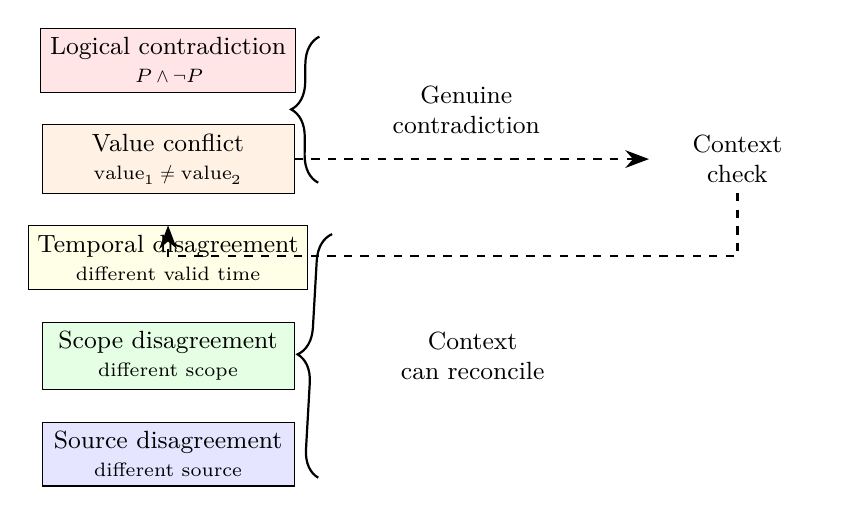
\begin{tikzpicture}[
    box/.style={rectangle, draw, minimum width=3.2cm, minimum height=0.7cm, align=center, font=\small},
    arrow/.style={-{Stealth[length=3mm]}, thick},
]

% Five contradiction types arranged vertically
\node[box, fill=red!10] (logical) {Logical contradiction\\[-1pt]\scriptsize $P \land \neg P$};
\node[box, fill=orange!10, below=0.4cm of logical] (value) {Value conflict\\[-1pt]\scriptsize $\mathrm{value}_1 \neq \mathrm{value}_2$};
\node[box, fill=yellow!10, below=0.4cm of value] (temporal) {Temporal disagreement\\[-1pt]\scriptsize different valid time};
\node[box, fill=green!10, below=0.4cm of temporal] (scope) {Scope disagreement\\[-1pt]\scriptsize different scope};
\node[box, fill=blue!10, below=0.4cm of scope] (source) {Source disagreement\\[-1pt]\scriptsize different source};

% Context dissolution bracket on the right
\draw[thick, decorate, decoration={brace, amplitude=10pt, mirror}]
    ($(temporal.east)+(0.3,0.3)$) -- ($(source.east)+(0.3,-0.3)$)
    node[midway, right=14pt, font=\small, align=center, text width=2.5cm] {Context\\can reconcile};

% Genuine contradiction bracket for top two
\draw[thick, decorate, decoration={brace, amplitude=10pt, mirror}]
    ($(logical.east)+(0.3,0.3)$) -- ($(value.east)+(0.3,-0.3)$)
    node[midway, right=14pt, font=\small, align=center, text width=2.5cm] {Genuine\\contradiction};

% Arrow showing context check flow
\node[right=4.5cm of value, font=\small, align=center, text width=2cm] (check) {Context\\check};
\draw[arrow, dashed] (value.east) -- (check.west);
\draw[arrow, dashed] (check.south) -- ++(0,-0.8) -| (temporal.north);

\end{tikzpicture}
\end{document}
